%https://chrisphan.com/2018/05/28/10-print-in-tikz/
\documentclass{standalone}

\usepackage{tikz}

\begin{document}

  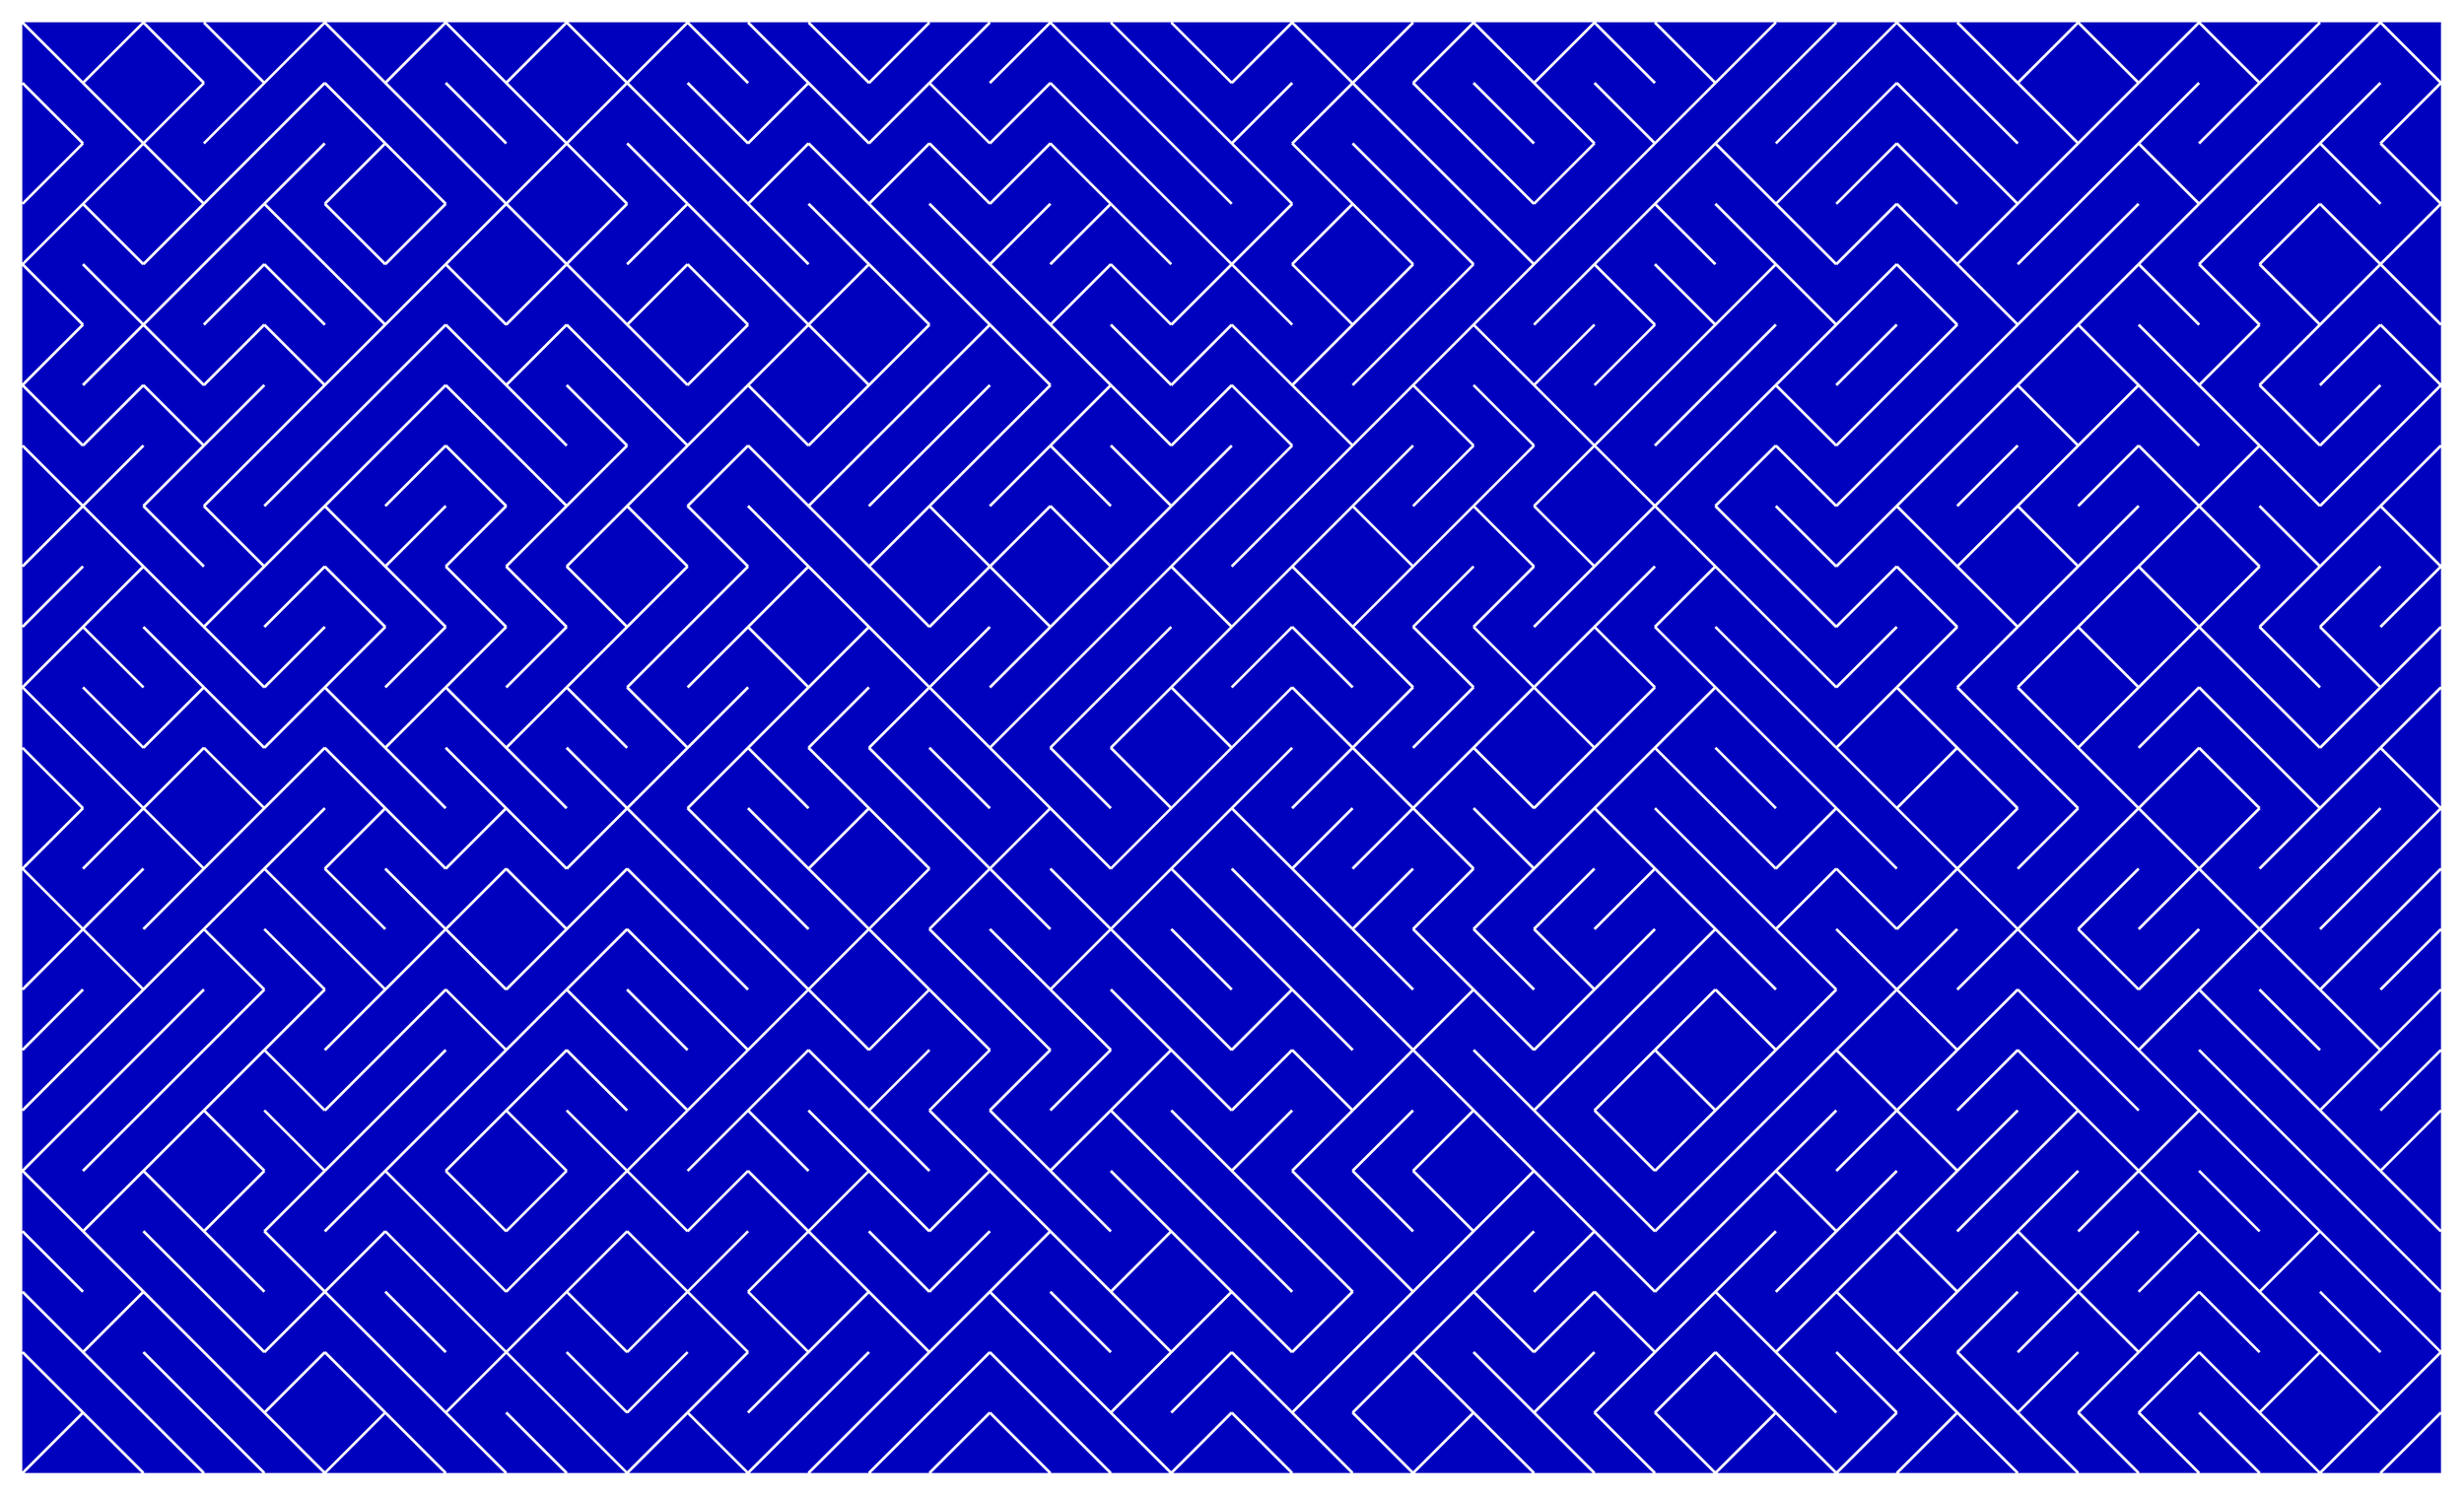
\begin{tikzpicture}

    % Draw background
    \fill[blue!75!black] (0, 0) -- (0, 24) --
    (40, 24) -- (40, 0) -- cycle;

    % Draw maze
    \foreach \y in {0, ..., 23}{
      \foreach \x in {0, ..., 39}{

        % Randomly choose a = 0 or a = 1
        \pgfmathrandominteger{\a}{0}{1};

        % If a = 0, then will draw SW-NE line
        % If a = 1, then will draw NW-SE line
        \draw[very thick, white] (\x, \y + \a)
          -- (\x + 1, \y + 1 - \a);
      }
    }

  \end{tikzpicture}

\end{document}